\documentclass[letterpaper]{article} % DO NOT CHANGE THIS
\usepackage[submission]{aaai2027}  % DO NOT CHANGE THIS
\usepackage[hyphens]{url}  % DO NOT CHANGE THIS
\usepackage{graphicx} % DO NOT CHANGE THIS
\urlstyle{rm} % DO NOT CHANGE THIS
\def\UrlFont{\rm}  % DO NOT CHANGE THIS
\usepackage{natbib}  % DO NOT CHANGE THIS AND DO NOT ADD ANY OPTIONS TO IT
\usepackage{caption} % DO NOT CHANGE THIS AND DO NOT ADD ANY OPTIONS TO IT
\frenchspacing  % DO NOT CHANGE THIS
\usepackage{algorithm}
\usepackage{algorithmic}
\usepackage{newfloat}
\usepackage{listings}
\usepackage{todonotes}
\usepackage{multirow}
\DeclareCaptionStyle{ruled}{labelfont=normalfont,labelsep=colon,strut=off} % DO NOT CHANGE THIS
\lstset{%
    basicstyle={\footnotesize\ttfamily},%
    numbers=left,numberstyle=\footnotesize,xleftmargin=2em,%
    aboveskip=0pt,belowskip=0pt,%
    showstringspaces=false,tabsize=2,breaklines=true}
\floatstyle{ruled}
\newfloat{listing}{tb}{lst}{}
\floatname{listing}{Listing}
\usepackage{booktabs}
\usepackage{amsmath}
\usepackage{amssymb}

\pdfinfo{
/TemplateVersion (2027.1)
}

\setcounter{secnumdepth}{2}

\title{REVEAL: A Rubric-Guided Agent for Explicit Evidence Sufficiency Verification in Long-Video Question Answering}
\author{Anonymous Submission}
\affiliations{}

\begin{document}

\maketitle

\begin{abstract}
Recently, retrieval- and memory-augmented agents have advanced long-video question answering by compressing each video into a searchable memory and retrieving evidence for a question on demand. However, these systems typically segment the video into fixed-length chunks that cut coherent scenes apart, and---whether the memory is then indexed as multi-scale summaries or multimodal knowledge graphs---they still equate retrieval relevance with evidence sufficiency, judging whether the collected evidence is enough only implicitly and often stopping to answer on segments that are related to the question yet cannot confirm or rule out the options. To address this, we propose REVEAL, a rubric-guided agent that explicitly verifies whether the retrieved evidence is sufficient for long-video question answering. Over a hierarchical video memory, REVEAL scores the retrieved evidence against automatically constructed, question-specific rubrics to judge whether each answer option can be confirmed or ruled out, and turns any unresolved option into a targeted repair query---so the search continues until the evidence is decisive rather than merely relevant. Training-free and using only a lightweight open Qwen model, REVEAL surpasses strong proprietary systems such as GPT-5 by 6.3 points on Video-MME-L and reaches state-of-the-art on multiple long-video benchmarks, showing that explicit sufficiency verification---rather than a heavier memory index such as a multimodal knowledge graph---is the key to reliable long-video reasoning.
\end{abstract}

% Uncomment after de-anonymized camera-ready release.
% \begin{links}
%     \link{Code}{https://anonymous.4open.science/r/rubric-video-repair}
% \end{links}

\section{Introduction}

Video large language models (video LLMs) are increasingly deployed in applications that must understand very long videos---AI glasses and home robots that perceive a user's day, assistants that search through hours of surveillance, meeting, or lecture recordings, and systems that answer questions about movies, sports broadcasts, or instructional footage~\citep{fu2024videomme,wang2024lvbench,zhou2024mlvu,tian2025egor1}. Long-video question answering (QA) is the canonical task for measuring this ability: a model must locate and reason over the few seconds of evidence that answer a question, buried in hours of otherwise redundant footage. The central obstacle is scale. Sampling even one frame per second from an hour-long video yields thousands of frames, far more than a vision-language model (VLM) can attend to at once; feeding them in directly exhausts both the visual-token budget and the context length of current models and inflates computational cost~\citep{qwen2_vl,gpt4o}. Specialized long-video models therefore shrink the visual input before or during encoding---through sparse frame sampling, keyframe selection, or visual-token compression that packs long clips into a fixed token budget~\citep{video_chatgpt,video_llava,llama_vid,chat_univi,longvu,sun2025videosalmonns}.

While such compression lets a model nominally cover a longer video, it is inherently lossy: sub-sampling frames or merging tokens throws away the fine-grained visual detail that many questions depend on, and the token cost still scales with duration. To avoid squeezing the whole video through the model, retrieval-augmented methods index the video into an external memory and, for each question, retrieve only a small set of relevant segments to reason over~\citep{lewis2020rag,karpukhin2020dpr,video_rag}. Because the model then conditions on a compact, query-specific subset instead of the entire stream, retrieval decouples reasoning cost from video length and scales gracefully to hours-long content.

However, retrieving from a flat pool of clips or captions has clear limits. A single-scale index treats every segment as an isolated unit: it cannot represent events that play out over different durations, and it offers no global view of how scattered moments connect into a storyline. Memory-augmented methods close part of this gap by processing the raw video into a structured memory before any question arrives---captioning segments, stacking them into hierarchical multi-scale summaries, or linking recurring entities into knowledge graphs---and pairing this memory with an agent that retrieves across levels over multiple rounds and decides on its own when to stop~\citep{moviechat,ma_lmm,fan2024videoagentmemory,worldmm,tian2025egor1,chen2025lvagent,wang2025avp}. This organizes a long temporal context into a searchable, multi-granularity memory and substantially improves long-video reasoning.

Yet across these designs a common blind spot persists: they treat retrieval relevance as evidence sufficiency. Consider a question that asks \emph{why} a woman leaves a restaurant. Retrieval readily surfaces the segment where she stands up and walks out---the closest match in both words and appearance---yet this clip shows only \emph{that} she leaves, not why, and can even mislead by suggesting she has simply finished her meal. The evidence that actually decides the question sits elsewhere and scores lower for relevance: an earlier moment in which she takes a phone call and looks alarmed. A system that stops at the most relevant clip answers from a distractor, whereas the \emph{sufficient} evidence is the segment that lets the model confirm the real cause and rule the misleading reading out. Compounding this, when a multi-round agent decides that it has ``seen enough,'' the judgment is implicit and holistic: it never names which option is still unresolved or which fact is missing, so follow-up queries stay broad and keep returning related but non-decisive clips. What is missing is an explicit account of whether the current evidence is sufficient to decide the question---and, when it is not, of exactly what to search for next.

We propose REVEAL, a rubric-guided agent that explicitly verifies whether the retrieved evidence is sufficient for long-video question answering, making this account an explicit step inside the inference loop. REVEAL first builds a hierarchical memory whose base units are scene segments formed by grouping visually similar frames---so a coherent event stays whole instead of being split at fixed time boundaries---and abstracts them upward into event- and video-level summaries for retrieval at multiple scales. Given a question, a rubric-guided verifier scores the retrieved evidence against a set of sufficiency criteria and judges, option by option, whether the evidence can confirm or rule it out; if any option remains undecided, the verifier emits a structured trace of what is missing, which a planner turns into a targeted repair query so the system searches for that specific gap rather than re-retrieving broadly. This retrieve--verify--repair loop continues until the evidence is decisive, and only then is an answer produced. Central to REVEAL is \emph{where} the rubric lives: rubrics have so far served mainly to grade final answers~\citep{liu2023geval,zheng2023judging,kim2023prometheus,es2023ragas} or to shape rewards in reinforcement learning~\citep{liu2025openrubrics,zhou2025ruscarl,zhang2026chasingtail}, whereas we move them into inference as a control signal that governs retrieval. To obtain the criteria without hand-crafting them, we design a construction pipeline that induces rubrics automatically from contrastive pairs of decisive versus misleading evidence, teaching the verifier the boundary between what settles a question and what merely looks relevant.

Our contributions are summarized as follows:
\begin{itemize}
    \item To our knowledge, we are the first to bring rubric-based evidence-sufficiency verification into the inference loop of long-video QA, recasting answering as an explicit retrieve--verify--repair process and opening a direction in which interpretable, criterion-level checks---rather than implicit confidence---govern when the collected evidence is enough.
    \item We design REVEAL, which couples a hierarchical, similarity-grouped video memory with a rubric-guided verifier that diagnoses per-option evidence gaps and repairs them through targeted retrieval, together with a pipeline that constructs the rubrics automatically from contrastive evidence pairs rather than manual authoring.
    \item REVEAL is training-free and uses only a lightweight open model, yet reaches state-of-the-art among comparable systems and surpasses strong proprietary models, scoring 78.9 on Video-MME-L ($+6.3$ over GPT-5) and 63.5 on LVBench.
\end{itemize}



\section{Related Work}

\subsection{Long Video Understanding}

Long-video understanding must reason over sparse evidence spread across a long temporal context, which is difficult to feed to an MLLM directly under visual-token and context-length budgets. Existing work therefore reduces the video input through sparse frame sampling, keyframe selection, or visual-token compression \citep{video_chatgpt,video_llava,llama_vid,chat_univi,longvu,sun2025videosalmonns}, or avoids full-video encoding by indexing the video into an external memory and retrieving a small set of relevant clips or memory items per question \citep{lewis2020rag,karpukhin2020dpr,video_rag,fan2024videoagentmemory,yeo2025worldmm,tian2025egor1}. Memory-based systems further structure this memory into captions, hierarchical multi-scale summaries, or entity knowledge graphs, and recent agentic methods add planning, tool use, and multi-round retrieval that continues until the agent judges it has gathered enough \citep{moviechat,ma_lmm,wang2024videoagentlongform,yang2024vca,chen2025lvagent,wang2025avp}. These systems improve access to relevant content, but relevance does not imply sufficiency, and their stopping decision is typically an implicit LLM or multi-agent judgment; in contrast, we make the sufficiency check explicit at the option and criterion level and use the resulting missing-evidence trace to steer the next retrieval.

\subsection{Rubric-based Methods}

Rubrics decompose a complex, subjective assessment into a set of explicit, verifiable criteria, separating the evaluation standard from the model that applies it. As LLM-as-a-judge scorers, rubrics turn a single holistic score into inspectable per-criterion judgments and have been used to evaluate open-ended, medical, and video outputs \citep{liu2023geval,zheng2023judging,kim2023prometheus,hashemi2024llmrubric,es2023ragas,arora2025healthbench,waheed2025videojudge,shaar2026movierecapsqa}, with recent work automating their construction at scale \citep{liu2026rubricssurvey,li2026rubrichub,zhou2026autochecklist,fan2025sedareval}. Beyond evaluation, rubrics have been used as reward signals in reinforcement learning, where an LLM grader supplies fine-grained feedback for tasks that lack ground-truth answers \citep{liu2025openrubrics,zhou2025ruscarl,zhang2026chasingtail}. In all of these settings, however, the rubric is applied to a completed answer---to score it or to reward it---rather than inside the reasoning process. We instead bring rubrics into the inference loop of a long-video agent, where they judge, option by option, whether the currently retrieved evidence is sufficient and expose which criteria remain unmet to drive the next retrieval.


\section{Methodology}

\begin{figure*}[t]
\centering
\includegraphics[width=\textwidth]{Figures/overview.pdf}
\caption{Overview of REVEAL. A long video is compressed into a \emph{hybrid} memory bank: a hierarchical narrative layer---segment-level captions (L1) stacked into event- and video-level summaries (L2, L3)---plus a visual keyframe layer and an online layer. Retrieval runs over the narrative text, while the answerer may additionally consult keyframes from the visual layer. At inference time, the planner decomposes the question into subqueries (round~0) or, guided by the verifier's missing-evidence trace, issues targeted or broadcast repair queries (round~$\ge 1$); the retriever collects timestamped multi-level evidence; and a rubric-guided verifier scores per-option sufficiency to decide whether the evidence is \texttt{SUFFICIENT} or \texttt{INSUFFICIENT}. Insufficient cases feed a repair trace back for another retrieval round, while sufficient cases---or a reached round budget---are passed to the answerer.}
\label{fig:arch}
\end{figure*}

REVEAL recasts long-video question answering as an explicit \emph{retrieve--verify--repair--answer} process (Figure~\ref{fig:arch}), built from three components. \textbf{(1)} A \emph{hybrid memory} compresses the video into a searchable bank: a hierarchical \emph{narrative} layer of scene-grouped captions and multi-scale summaries, together with a \emph{visual} keyframe layer and an \emph{online} layer (Section~\ref{sec:memory}). \textbf{(2)} An offline \emph{rubric-construction} pipeline induces the verifier's criteria from contrastive pairs of decisive and misleading evidence, so the rubrics are built automatically rather than by hand (Section~\ref{sec:rubric}). \textbf{(3)} A rubric-guided \emph{retrieve--verify--repair} loop then, given a question, retrieves candidate evidence, scores its sufficiency for every option with a verifier, and---when the evidence is insufficient---turns the verifier's missing-evidence trace into targeted repair queries, iterating until the evidence is decisive before an answer is produced (Section~\ref{sec:loop}). A single open LLM serves as the planner, verifier, and answerer, and retrieval is performed over text. We detail each component below.

\subsection{Hybrid Memory Construction}
\label{sec:memory}

Retrieval quality is bounded by how the video is segmented and indexed: fixed-length chunks split a coherent scene across several units, and a single-scale index cannot serve questions that range from a one-second action to a whole-video summary. Given a long video $V$, REVEAL builds a \emph{hybrid} memory with three layers: a hierarchical \emph{narrative} layer whose base units follow scene boundaries rather than a fixed clock and are summarized upward for retrieval at multiple scales; a \emph{visual} layer of representative keyframes; and an \emph{online} layer that can regenerate captions from raw frames on demand. The narrative layer is the retrieval backbone: all retrieval is over its text embeddings, and answer-relevant visual content is written into its captions. The visual layer additionally holds keyframes that the answerer can optionally consume---which we enable on egocentric benchmarks, where fine visual detail matters---and the online layer is retained for on-demand re-captioning.

\paragraph{L1: segment-level narrative memory.}
We sample video frames at 1 fps and remove low-quality frames before chunking. Near-black, near-white, or nearly uniform frames are filtered using JPEG size and pixel statistics, and blurred frames are removed with a Laplacian-variance criterion. The remaining frames are encoded by SigLIP~\citep{zhai2023siglip}. Adjacent frames are greedily grouped into variable-length shot-like segments when their visual cosine similarity exceeds a threshold $\theta$; we use $\theta=0.8$ by default. For each segment, a VLM generates a caption from the segment frames and the temporally aligned subtitle or speech transcript when available. The caption is instructed to preserve answer-discriminative details, including identities, objects, actions, state changes, temporal transitions, spatial relations, and counts. This produces an L1 memory item of roughly 10 seconds on average:
\begin{equation}
    c_i^{(1)}=(t_i^s,t_i^e,x_i^{(1)},K_i),
\end{equation}
where $(t_i^s,t_i^e)$ are temporal boundaries, $x_i^{(1)}$ is the segment-level narrative, and $K_i$ stores representative keyframes (the visual layer). Retrieval never uses these keyframes directly---it operates on the caption text $x_i^{(1)}$, into which visual content has been written---but the answerer may optionally consume the keyframes of the selected segments.

\paragraph{L2 and L3: stacked summaries.}
Upper levels are built by textual stacking rather than by re-captioning video frames. Every 12 consecutive L1 items are summarized by an LLM into a 120-word L2 event-timeline summary. Every 12 consecutive L2 items are then summarized into a 300-word L3 video-level summary. Formally,
\begin{equation}
    x_j^{(2)}=S_2(x_{12j}^{(1)},\ldots,x_{12j+11}^{(1)}),
\end{equation}
\begin{equation}
    x_k^{(3)}=S_3(x_{12k}^{(2)},\ldots,x_{12k+11}^{(2)}),
\end{equation}
where $S_2$ and $S_3$ denote LLM summarizers with prompts that retain temporal order and answer-relevant entities. L2 captures event processes, while L3 captures global themes and coarse temporal structure. This stacked construction keeps upper-level memories consistent with L1 observations and avoids additional visual-processing cost.

\paragraph{Text embedding and online memory.}
Each textual memory item $x_i^{(\ell)}$ from level $\ell\in\{1,2,3\}$ is encoded by BGE-M3~\citep{chen2024bgem3}:
\begin{equation}
    \mathbf{h}_i^{(\ell)}=f_{\mathrm{text}}(x_i^{(\ell)}).
\end{equation}
The offline memory bank is therefore
\begin{equation}
    \mathcal{M}=\mathcal{M}^{(1)}\cup\mathcal{M}^{(2)}\cup\mathcal{M}^{(3)}.
\end{equation}
The memory format can additionally retain the raw frames around each segment. Using them, we explored an \emph{online} layer $\mathcal{M}^{+}$ that, when the verifier repeatedly reports missing fine-grained evidence, returns to the original frames around candidate timestamps and regenerates captions for the requested detail as additional textual evidence. On the long-video benchmarks we study, this did not improve accuracy: the dominant failure mode is retrieval \emph{recall} over the offline bank rather than caption incompleteness. The default system therefore disables online supplementation and performs all evidence repair through additional text retrieval over $\mathcal{M}$; we retain the raw frames only as an interface for future work.

\subsection{Contrastive Rubric Construction}
\label{sec:rubric}

The verifier needs criteria that separate decisive evidence from merely relevant context, but writing such criteria by hand for every question type is costly, subjective, and hard to calibrate. We instead construct them automatically---before inference---from contrastive evidence pairs that distinguish sufficient evidence from misleading but insufficient evidence. Construction uses only training or development questions with known answers; test answer labels are never used. Figure~\ref{fig:rubric_construction} illustrates the pipeline.

\begin{figure*}[t]
\centering
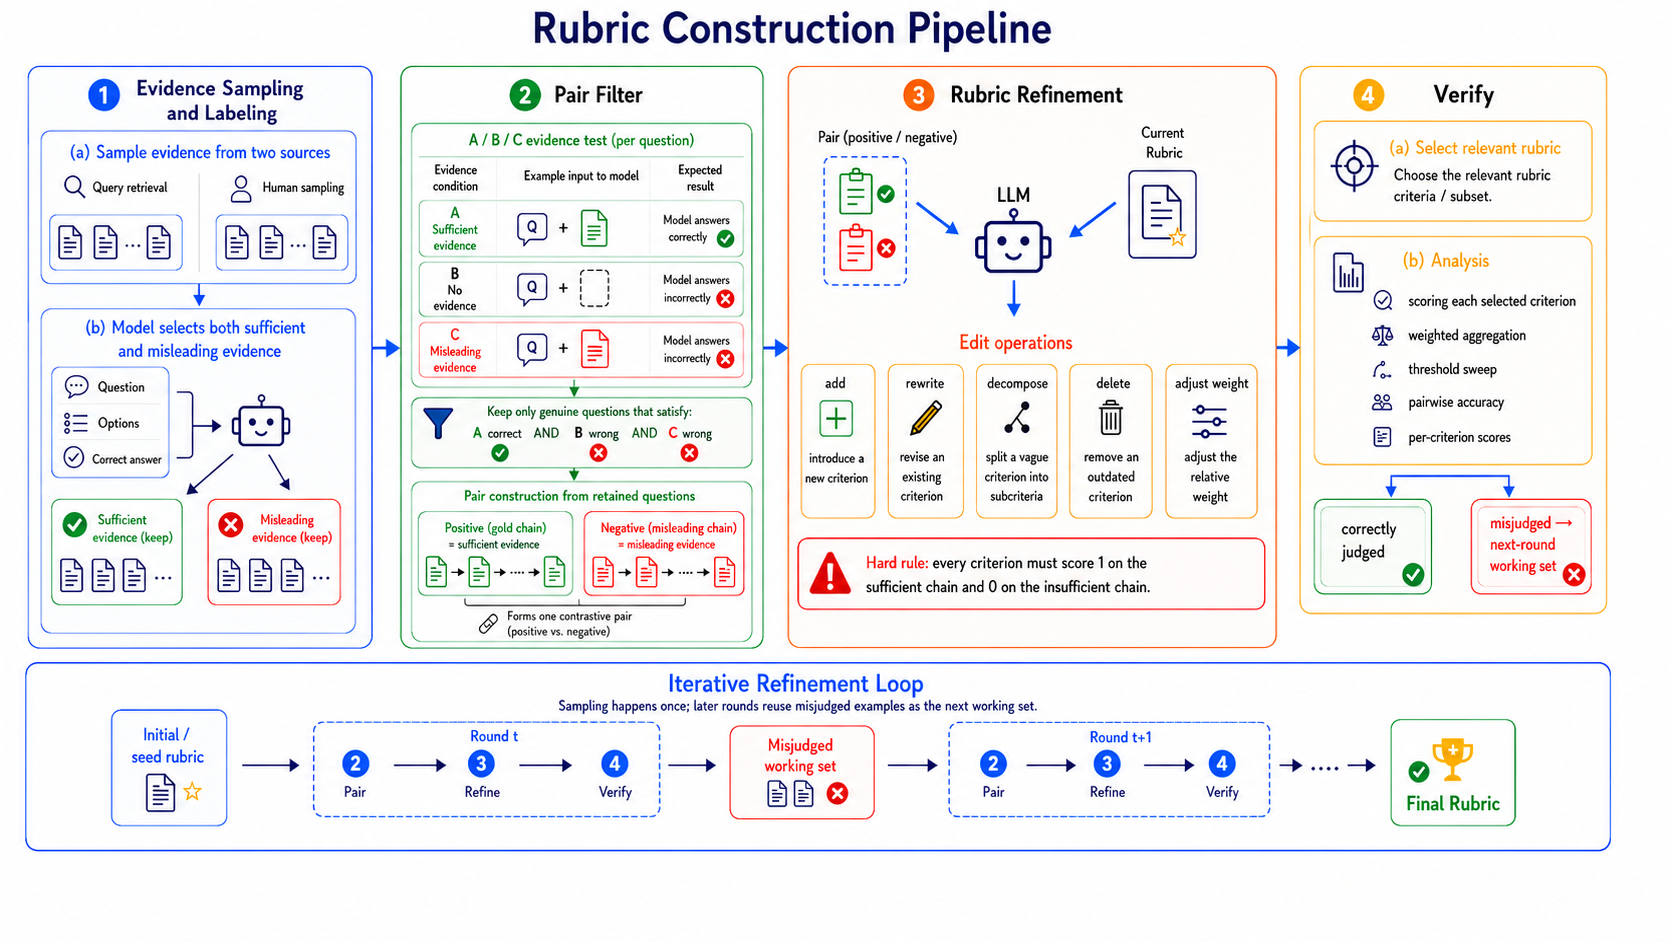
\includegraphics[width=\textwidth]{Figures/rubric_construction.png}
\caption{Contrastive rubric construction pipeline. We first sample and label candidate evidence sets, then retain only genuine questions that satisfy the A/B/C evidence test: gold evidence answers correctly, no evidence answers incorrectly, and misleading evidence answers incorrectly. Each retained gold--misleading pair is used to refine the current type-specific rubric through add, rewrite, decompose, delete, and weight-adjustment operations. The refined rubric is verified on held-out examples, and misjudged cases are carried into the next refinement round.}
\label{fig:rubric_construction}
\end{figure*}

\paragraph{Candidate evidence pool.}
For each training question, we first retrieve a broad textual pool from the hierarchical memory: L1@16, L2@16, and all L3 summaries. This pool is large enough to contain both decisive evidence and hard distractors, but small enough for an LLM to inspect in a single construction step.

\paragraph{Gold and misleading evidence selection.}
A teacher model is given the question, answer options, gold answer, and the candidate pool. It selects a minimal gold subset $E^{+}$ that is sufficient to force the correct answer. The subset must be compact and decisive: removing its key evidence should make the answer ambiguous. The same teacher also selects a misleading subset $E^{-}$ from the pool. This subset should appear relevant to the question but omit the decisive fact, temporal transition, or exclusion evidence, thereby leading the answer model toward an incorrect or unsupported option.

\paragraph{Closed-book filtering.}
We retain a contrastive pair only if three answering tests hold: the answer model answers correctly with $E^{+}$, answers incorrectly without evidence, and answers incorrectly with $E^{-}$. This filter removes questions that can be solved from language priors alone and removes pairs whose misleading evidence is not actually misleading. In our Video-MME construction, this filtering discards approximately 44\% of candidate questions, indicating that prior-answerable examples are a major source of noise for rubric induction.

\paragraph{Online type-specific refinement.}
For each retained pair $(E^{-},E^{+})$, the proposer LLM receives the current rubric for the corresponding question type and edits it in place. The allowed operations are \textsc{Add}, \textsc{Rewrite}, \textsc{Decompose}, \textsc{Delete}, and \textsc{AdjustWeight}. \textsc{Add} introduces a missing criterion, \textsc{Rewrite} clarifies a criterion, \textsc{Decompose} splits a multi-aspect criterion into independently scorable checks, \textsc{Delete} removes redundant or non-discriminative criteria, and \textsc{AdjustWeight} changes the weight according to how strongly the criterion separates $E^{+}$ from $E^{-}$. Refinement is serial within each question type, with inline deduplication and weight normalization after each batch. The result is a set of type-level weighted rubrics used by the inference-time verifier. Figure~\ref{fig:rubric_example} shows an excerpt of a constructed rubric.

\begin{figure}[t]
\centering
\small
\setlength{\tabcolsep}{5pt}
\renewcommand{\arraystretch}{1.25}
\begin{tabular}{@{}p{0.95\columnwidth}@{}}
\toprule
\multicolumn{1}{@{}l@{}}{\textbf{Rubric for \emph{Counting} questions}\quad(``How many $X$ occur?'',\ $\tau\!=\!0.8$)} \\
\midrule
\textbf{C1. Is each distinct instance explicitly enumerated?} \hfill (w$=$5) \newline
\textbf{[1.0]} evidence names/distinguishes every instance to be counted;\ \
\textbf{[0.5]} a quantity is implied but instances are not separated;\ \
\textbf{[0]} only generic mentions (``several'', ``many''). \\
\textbf{C2. Is each instance identified by a defining attribute?} \hfill (w$=$4) \newline
\textbf{[1.0]} a marker (label, logo, on-screen text) classifies each instance;\ \
\textbf{[0.5]} markers are partial/ambiguous;\ \ \textbf{[0]} none. \\
\textbf{C3. Is the evidence consistent enough to exclude wrong counts?} \hfill (w$=$4) \newline
\textbf{[1.0]} consistent, competing counts are ruled out;\ \
\textbf{[0.5]} partly;\ \ \textbf{[0]} contradictory / cannot exclude. \\
\midrule
\multicolumn{1}{@{}p{0.95\columnwidth}@{}}{$\rho=\tfrac{\sum_k w_k z_k}{\sum_k w_k}$;\ \ evidence is \textsc{sufficient} only if $\rho\!\ge\!\tau$ \emph{and} exactly one option scores \emph{true}.} \\
\bottomrule
\end{tabular}
\caption{An automatically constructed rubric for one question type. Each criterion is a concrete yes/partial/no check with an explicit decision boundary (score $1/0.5/0$); the type-specific criteria (C1--C2) carry the heaviest weight because they capture what makes evidence \emph{decisive} for counting. The weighted score $\rho$ is gated by the per-type threshold $\tau$. General criteria shared by all types (coverage, specificity, consistency; $\tau\!=\!0.6$) are omitted for space.}
\label{fig:rubric_example}
\end{figure}

\subsection{Rubric-guided Retrieve--Verify--Repair}
\label{sec:loop}

Using the constructed rubrics, REVEAL answers each question through an iterative loop driven by a planner. Given the question and options $O=\{o_1,\ldots,o_m\}$, the planner first decomposes the question into retrieval queries; a verifier then scores whether the retrieved evidence is sufficient to decide every option; and, if not, the planner turns the verifier's missing-evidence trace into repair queries for the next round. An answer is produced only once the evidence is decisive. We describe the four stages in turn.

\paragraph{Query decomposition and retrieval.}
A single question embedding tends to match high-level topical content and miss the decisive local moment. At round~0, therefore, the planner decomposes the question and options into 2--4 atomic subqueries, each self-contained and short (typically $\le 15$ words). For a subquery $u$, retrieval uses only BGE-M3 text similarity,
\begin{equation}
    s(u,c_i^{(\ell)})=\cos(f_{\mathrm{text}}(u),\mathbf{h}_i^{(\ell)}),
\end{equation}
run independently on L1, L2, and L3 (default capacity L1@8, L2@4, L3@2 per round). Candidates from all levels and subqueries are merged into one pool, deduplicated by text similarity and timestamp overlap, and sorted by score, so the verifier sees evidence at multiple temporal scales: L1 supplies local detail, L2 event processes, and L3 global context.

\paragraph{Rubric-guided verification.}
Multi-round agents usually judge that they have ``seen enough'' with a single holistic decision, which cannot say which option is unresolved or which requirement is unmet, and so conflates relevance with sufficiency. REVEAL instead applies an explicit, per-criterion check---the central component of our framework---scoring, for every option, whether the evidence is adequate to confirm or rule it out rather than whether the option is likely correct. The rubric combines general criteria with question-type-specific criteria, each of the form
\begin{equation}
    r_k=(\mathrm{name},\mathrm{description},b_k^1,b_k^{0.5},b_k^0,w_k),
\end{equation}
where $b_k^1$, $b_k^{0.5}$, $b_k^0$ define the scoring boundaries for full, partial, and missing evidence, and $w_k$ is the criterion weight. General criteria cover broad requirements (coverage, specificity, consistency, temporal grounding); type-specific criteria specialize them for temporal-order, object-state, action, counting, spatial-relation, and causal questions. For each option $o_j$ and criterion $r_k$, the verifier assigns $z_{jk}\in\{1,0.5,0\}$ according to whether the evidence is sufficient to \emph{judge} that option under the criterion---evidence that clearly rules the option out scores as high as evidence that confirms it---giving an option-level sufficiency score
\begin{equation}
    \rho_j=\frac{\sum_k w_k z_{jk}}{\sum_k w_k}.
\end{equation}
In the same pass the verifier emits a direct judgment $\hat{y}_j\in\{\texttt{true},\texttt{false},\texttt{unknown}\}$, which we gate by the sufficiency score, forcing any option whose evidence is not sufficient to \texttt{unknown}:
\begin{equation}
    y_j=\begin{cases}
    \hat{y}_j,     & \rho_j\ge\tau,\\
    \texttt{unknown}, & \rho_j<\tau.
    \end{cases}
\end{equation}
Here \texttt{false} matters as much as \texttt{true}: sufficient evidence may rule an option out rather than support it. The threshold $\tau$ is set per rubric and tuned on development questions: general criteria use $\tau=0.6$ and type-specific rubrics use $\tau=0.8$. REVEAL declares the evidence \texttt{SUFFICIENT} only when exactly one option is \texttt{true} and all others are \texttt{false}; otherwise it is \texttt{INSUFFICIENT}, and the verifier reports the unresolved options, weak criteria, and a concise missing-evidence analysis.

\paragraph{Repair planning.}
When the evidence is insufficient, the planner conditions on this verifier trace rather than only on the original question, and chooses between two strategies. The \textit{targeted} strategy generates focused queries for the missing facts, such as an action before an object appears, the outcome after a scene transition, or the order between two events. The \textit{broadcast} strategy samples temporally diverse memories along the timeline, for overview or chronological questions or when targeted retrieval has failed. To avoid repeated search, a new query is discarded if it is highly redundant with previous queries (Jaccard overlap) or already covered by the current evidence (BGE-M3 similarity); if all targeted queries are discarded, the planner falls back to broadcast. The loop runs for at most three rounds by default.

\paragraph{Answer generation.}
By the time the loop stops, the pool also holds many related-but-redundant segments that can drown out the few decisive ones if fed verbatim. REVEAL therefore reorders the \emph{entire} accumulated pool with a rubric-guided rerank---the LLM ranks segments by how well they satisfy the question's rubric, so decisive segments come first and near-duplicates sink---and passes the reordered pool \emph{in full}, without truncation, to the answerer, question first. The answerer is the same open LLM at temperature~0; it reads the reranked narrative evidence and, optionally, the keyframes of the selected segments (enabled on egocentric benchmarks, where fine visual detail helps). If the loop stops without full sufficiency, the answerer still returns the best-supported option for benchmark compatibility, while the system records the missing-evidence statement for analysis.

\section{Experiments}


\begin{table*}[t]
\centering
\scriptsize
\setlength{\tabcolsep}{3.0pt}
\renewcommand{\arraystretch}{1.08}
\resizebox{\textwidth}{!}{%
\begin{tabular}{llcccccccc}
\toprule
Category & Method & Size
& EgoLifeQA
& Ego-R1 Bench
& LVBench
& MLVU
& Video-MME (long)
& LongVideoBench (val)
& Avg. \\
\midrule

General-purpose MLLMs
& Qwen3-VL-8B$^{\dagger\S}$
& 8B
& 38.6 & 35.7 & 48.3 & 61.0 & 67.6 & $-$ & $-$ \\

& Gemini 2.5 Pro$^{\dagger\S}$
& $-$
& 46.4 & 46.7 & 57.0 & 55.7 & 69.8 & $-$ & $-$ \\

& GPT-5$^{\dagger\S}$
& $-$
& 48.6 & 46.3 & 60.4 & 74.3 & 72.6 & $-$ & $-$ \\

\midrule

Specialized Long-video Models
& VideoChat-Flash$^{\dagger\S}$
& 7B
& 34.2 & 42.7 & 33.2 & 74.7 & 44.1 & 64.7 & $-$ \\

& Video-RTS$^{\dagger\S}$
& 7B
& 48.2 & 47.4 & 39.8 & $-$ & 47.9 & 56.6 & $-$ \\

& video-SALMONN S$^{\dagger\S}$
& 8B
& $-$ & $-$ & 55.6 & $-$ & 71.3 & $-$ & $-$ \\

& LongVideo-R1$^{\dagger\S}$
& 8B
& $-$ & $-$ & 60.7 & 71.3 & 58.0 & $-$ & $-$ \\

& FlexMem (LLaVA-Video-7B)$^{\dagger\S}$
& 7B
& $-$ & $-$ & 51.0 & 72.4 & 54.4 & 63.6 & $-$ \\

\midrule

Retrieval-augmented Methods
& Video-RAG$^{\ddagger}$
& $-$
& $-$ & $-$ & $-$ & $-$ & 66.44 & $-$ & $-$ \\

& HippoRAG 2$^{\ddagger}$
& $-$
& $-$ & $-$ & $-$ & $-$ & $-$ & $-$ & $-$ \\

& Vgent$^{\ddagger}$
& $-$
& $-$ & $-$ & $-$ & $-$ & $-$ & $-$ & $-$ \\

\midrule

Memory-augmented Methods
& Ego-R1$^{\dagger\S}$
& 3B
& 53.0 & 52.0 & 34.1 & $-$ & 42.7 & $-$ & $-$ \\

& M3-Agent$^{\dagger\S}$
& 7B
& 53.5 & 52.0 & 49.3 & $-$ & 55.3 & $-$ & $-$ \\

& VideoLucy$^{\ddagger}$
& $-$
& $-$ & $-$ & $-$ & $-$ & $-$ & $-$ & $-$ \\

& WorldMM$^{\ddagger}$
& $-$
& 65.6 & 65.3 & 61.9 & $-$
& 58.67\,(76.6) & $-$ & $-$ \\

\midrule

& \textbf{Ours}
& $-$ & 60.00 & 62.4& 63.54 & $-$ & \textbf{78.89} & $-$ & $-$ \\


\bottomrule
\end{tabular}%
}
\caption{
Main comparison on six public long-video reasoning benchmarks.
Methods within each category are ordered chronologically according to their
first public release.
LongVideoBench results are evaluated on its public validation split.
The \emph{Size} column reports the parameter scale of the fixed model or
checkpoint used for evaluation.
For proprietary MLLMs, ``--'' indicates that the model size is undisclosed.
For modular retrieval- and memory-augmented frameworks, ``--'' indicates that
the framework does not prescribe a single task-specific trained backbone.
We instantiate their replaceable reasoning or controller LLM with Qwen3.5-27B,
while preserving the original video preprocessing, indexing, memory
construction, retrieval, perception, and iterative reasoning procedures.
For methods with officially released task-specific checkpoints, such as
Ego-R1 and M3-Agent, we directly use the released models and report their
original results without replacing the trained controller.
$^{\dagger}$ denotes previously reported results.
$^{\ddagger}$ denotes results evaluated by us using Qwen3.5-27B as the
replaceable reasoning or controller LLM.
$^{\S}$ indicates that some target benchmarks were not originally reported
and require additional evaluation using the released checkpoint, official
implementation, or official API.
Parenthesized results denote the result reported with the proprietary
controller used in the corresponding paper.
The average is calculated only when results on all six benchmarks are available.
}
\label{tab:main_results}
\end{table*}


\begin{table*}[t]
\centering
\scriptsize
\setlength{\tabcolsep}{3.0pt}
\renewcommand{\arraystretch}{1.08}
\resizebox{\textwidth}{!}{%
\begin{tabular}{llccccccc}
\toprule
Category & Method & 
& EgoLifeQA
& Ego-R1 Bench
& LVBench
& Video-MME (long)
& LongVideoBench (val)
& Avg. \\
\midrule

MLLMs

& Qwen3-VL-8B$^{\dagger\S}$
& 8B & 38.6 & 35.7 & 48.3 & 61.0 & 67.6 & $-$ \\

& Gemini 2.5 Pro$^{\dagger\S}$
& $-$ & 46.4 & 46.7 & 57.0 & 55.7 & 69.8 & $-$ \\

& GPT-5$^{\dagger\S}$
& $-$ & 48.6 & 46.3 & 60.4 & 74.3 & 72.6 & $-$ \\

\midrule
Long Video LLMs
& VideoChat-Flash$^{\dagger}$
& 7B & 34.2 & 42.7 & 33.2 & 44.1 & 64.7 & 48.9 \\

& Video-RTS$^{\dagger\S}$
& 7B & 48.2 & 47.4 & 39.8 & 47.9 & 56.6 & $-$ \\

& video-SALMONN S$^{\dagger\S}$
& 8B & $-$ & $-$ & 55.6 & 71.3 & $-$ & $-$ \\

& FlexMem (LLaVA-Video-7B)$^{\dagger\S}$
& 7B & $-$ & $-$ & 51.0 & 54.4 & 63.6 & $-$ \\

\midrule
RAG-based Video LLMs
& LightRAG$^{\ddagger}$
& $-$ & $-$ & $-$ & $-$ & $-$ & $-$ & $-$ \\

& Video-RAG$^{\ddagger}$
& $-$ & $-$ & $-$ & $-$ & 66.44 & $-$ & $-$ \\

& HippoRAG 2$^{\ddagger}$
& $-$ & $-$ & $-$ & $-$ & $-$ & $-$ & $-$ \\

\midrule
Memory-based Video LLMs

& HippoMM$^{\ddagger}$
& $-$ & $-$ & $-$ & $-$ & $-$ & $-$ & $-$ \\

& Ego-R1$^{\dagger\S}$
& 3B & 53.0 & 52.0 & 34.1 & 42.7 & $-$ & $-$ \\

& M3-Agent$^{\dagger\S}$
& 7B & 53.5 & 52.0 & 49.3 & 55.3 & $-$ & $-$ \\

& WorldMM$^{\ddagger}$
& $-$ & (65.6) & (65.3) & (61.9) &  58.67(76.6) & $-$ & $-$ \\


\addlinespace[2pt]
& \textbf{Ours}
& $-$ & 60.00 & $-$ & 63.54 & \textbf{78.89} & $-$ & $-$ \\

\bottomrule
\end{tabular}%
}
\caption{
Main comparison on five public long-video reasoning benchmarks.
Methods within each category are ordered chronologically according to their
first public release.
LongVideoBench results are evaluated on its public validation split.
The \emph{Size} column reports the parameter scale of the fixed model or
checkpoint used for evaluation.
For proprietary MLLMs, ``--'' indicates that the model size is undisclosed.
For RAG-based and memory-based training-free frameworks, ``--'' indicates that
no task-specific trained backbone is used; we instantiate their separable
reasoning or controller LLM with Qwen3.5-27B while preserving the original
video processing, memory construction, retrieval, perception, and tool-use
components.
$^{\dagger}$ denotes results reported in the original paper or obtained from
an existing unified evaluation.
$^{\ddagger}$ denotes results evaluated by us using Qwen3.5-27B as the
reasoning or controller LLM.
$^{\S}$ indicates that some target benchmarks were not reported and require
additional evaluation using the released checkpoint, official implementation,
or official API.
The average is calculated only when results on all five benchmarks are available.
}
\label{tab:main_results}
\end{table*}


\subsection{Experimental Setup}

\paragraph{Benchmarks.}
We evaluate on five public long-video understanding benchmarks: EgoLifeQA, Ego-R1 Bench, LVBench, MLVU, and Video-MME-L. Video-MME-L evaluates multiple-choice question answering over long videos and is widely used in recent long-video studies. LVBench focuses on reasoning over extended temporal contexts. MLVU provides a multi-task long-video evaluation suite; we use its multiple-choice setting to match our answer-selection formulation. EgoLifeQA and Ego-R1 Bench focus on egocentric long-video reasoning, where task-relevant evidence is sparse, temporally distributed, and often tied to fine-grained daily-life events. This benchmark set covers both third-person and egocentric videos, while keeping all evaluation data publicly accessible.

\paragraph{Baselines.}
We compare REVEAL with four groups of recent long-video systems, following Table~\ref{tab:main_results}. 
\textbf{MLLMs} directly process sampled video frames with strong multimodal language models, including Qwen3-VL-8B, Gemini 2.5 Pro, and GPT-5.
\textbf{Long Video LLMs} are models designed or adapted for long-video understanding, including VideoChat-Flash, Video-RTS, and video-SALMONN S.
\textbf{RAG-based Video LLMs} retrieve relevant video evidence before answering, including HippoRAG~2, Video-RAG, and Vgent with Qwen3.5-27B as the reasoning model when the released implementation supports model replacement.
\textbf{Memory Agents} build structured or agentic memories over long videos, including HippoMM, M3-Agent, WorldMM, and VideoARM with Qwen3.5-27B as the backend reasoner where applicable. Our method is listed as a rubric-guided agent using the same Qwen3.5-27B answer model.

We also construct controlled internal variants for the ablation study on Video-MME-L and LVBench. These variants share the same answer model and differ only in retrieval round, rubric-based sufficiency verification, and multi-level memory usage. This controlled design separates the effects of iterative search, explicit evidence sufficiency judgment, and hierarchical memory across the primary benchmark and an additional long-video benchmark from Table~\ref{tab:main_results}.

\paragraph{Implementation Details.}
Unless otherwise stated, all controlled variants use the same answer model, frame rate, chunking procedure, and retrieval budget per round. The default maximum number of retrieval-repair rounds is $K=3$. The verifier sufficiency threshold $\tau$ is set per rubric and tuned on development questions: general criteria use $\tau=0.6$ and type-specific rubrics use $\tau=0.8$. For multi-level retrieval, each round retrieves evidence from local segment memories, event-level summaries, and video-level summaries. For single-level retrieval, only the local segment memory is used.

\subsection{Main Results}

Table~\ref{tab:main_results} compares REVEAL with recent long-video systems across the five benchmarks. The results are organized by method category, including direct MLLMs, long-video LLMs, RAG-based video LLMs, memory agents, and our rubric-guided agent. Direct MLLMs provide strong general multimodal reasoning, but they must compress long videos through sparse frame sampling. Retrieval-augmented and memory-based methods are more suitable for long videos because they organize long temporal contexts into searchable evidence. However, these methods still mainly rely on semantic relevance or implicit self-reflection, so they may retrieve clips that are related to the question but insufficient for deciding the answer. REVEAL targets this limitation by verifying whether the retrieved evidence is sufficient to judge each option, then using the resulting diagnostic trace to repair missing evidence.


\begin{table}[t]
\centering
\scriptsize
\setlength{\tabcolsep}{2.5pt}
\renewcommand{\arraystretch}{1.05}
\resizebox{\columnwidth}{!}{%
\begin{tabular}{lccccc}
\toprule
\multirow{2}{*}{\textbf{Method}}
& \multicolumn{3}{c}{Components}
& \multicolumn{2}{c}{Datasets} \\
\cmidrule(lr){2-4}
\cmidrule(lr){5-6}
& \shortstack{Iter.\\Ret.}
& \shortstack{Rubric\\Suff.}
& \shortstack{Hybrid\\Mem.}
& \shortstack{Video-\\MME-L}
& LVBench \\
\midrule

$\mathcal{M}_{\mathrm{base}}$
&  &  &  & 65.89 & $-$ \\

$\mathcal{M}_{\mathrm{iter}}$
& \checkmark &  &  & 72.78 & $-$ \\

$\mathcal{M}_{\mathrm{iter+rubric}}$
& \checkmark & \checkmark &  & 75.22 & $-$ \\

$\mathcal{M}_{\mathrm{iter+hybrid}}$
& \checkmark &  & \checkmark & 77.67 & $-$ \\

\textbf{Ours}
& \checkmark
& \checkmark
& \checkmark
& \textbf{78.89}
& $-$ \\
\bottomrule
\end{tabular}%
}
\caption{Ablation results on Video-MME-L and LVBench.
$\mathcal{M}_{\mathrm{base}}$ uses single-round retrieval over local
segment memory. $\mathcal{M}_{\mathrm{iter}}$ adds iterative retrieval.
The rubric and hybrid variants further introduce rubric-based
sufficiency verification and hybrid memory, respectively. Ours combines
all three components.}
\label{tab:ablation_design}
\end{table}

\subsection{Ablation Study}

Table~\ref{tab:ablation_design} reports the controlled ablation results on Video-MME-L and LVBench. Video-MME-L is the primary ablation setting, while LVBench serves as an additional benchmark from the main comparison to test whether the component effects transfer beyond a single dataset. We isolate three design factors: multi-round retrieval, rubric-based evidence sufficiency verification, and multi-level memory retrieval. All variants use the same answer model and comparable per-round retrieval budget.

\paragraph{Effect of Multi-round Retrieval.}
The single-round baseline achieves 65.89 on Video-MME-L. Replacing one-shot retrieval with multi-round single-level retrieval raises performance to 72.78, a gain of 6.89 points. This shows that long-video QA benefits from iterative evidence seeking: the system can revise its query after the first retrieval result instead of committing to a fixed top-ranked evidence set.

\paragraph{Effect of Rubric-based Sufficiency Verification.}
Adding rubric-based sufficiency verification to the multi-round single-level setting improves performance from 72.78 to 75.22. The gain indicates that the verifier is not merely adding another reasoning call; it provides an explicit criterion for deciding whether the current evidence can determine each option. With rubric-guided decomposition, the planner receives more precise missing-evidence targets and avoids repeatedly retrieving topically relevant but non-decisive segments.

\paragraph{Effect of Multi-level Memory.}
Using multi-level memory without rubric verification reaches 77.67, outperforming the single-level variants. This confirms that hierarchical memory is important for long videos: local segment memories preserve fine-grained details, event-level memories capture temporal processes, and paragraph-level summaries provide global context. The full model combines multi-round retrieval, rubric-based sufficiency verification, and multi-level memory, reaching 78--79 on Video-MME-L. The improvement over the multi-level no-rubric variant suggests that better memory coverage and explicit evidence sufficiency checking are complementary.


\subsection{Analysis}

\begin{figure}[t]
\centering
\includegraphics[width=\columnwidth]{Figures/evidence_volume.pdf}
\caption{Accuracy versus evidence \emph{volume} on Video-MME-L. The curve strips the pipeline to a single dense query over segment captions and feeds the answerer its top-$N$ most relevant segments (no decomposition, no multi-level memory, no rubric verification), sweeping $N$ from $8$ to $512$. Accuracy saturates at $64$ segments ($75.7\%$) and then plateaus---even declines---as more relevant segments are added. REVEAL (star) reaches $78.9\%$ with only ${\sim}39$ \emph{verified} segments, above the best volume-only budget by $3.2$ points and every larger budget by ${\sim}5$. More relevant evidence is not the lever; verified sufficiency is.}
\label{fig:volume}
\end{figure}

\paragraph{Is more evidence all you need?}
A natural objection to an explicit verifier is that its gains could be had more cheaply by simply retrieving more evidence. Figure~\ref{fig:volume} tests this directly. We reduce the system to a single dense query over the segment captions and feed the answerer its top-$N$ most relevant segments, sweeping $N$ from $8$ to $512$; a typical Video-MME-L video holds a few hundred segments, so this scans from scarce to near-exhaustive evidence. Accuracy climbs while evidence is scarce, but saturates at $64$ segments ($75.7\%$) and then plateaus and even dips as more relevant segments are added---beyond a point, additional captions dilute rather than sharpen the decisive evidence, filling the answerer's context with topically related but non-decisive text. This brute-force ceiling stays $3.2$ points below REVEAL ($78.9\%$), which uses only about $39$ segments---fewer than the volume baseline needs even to reach its own peak. The bottleneck is therefore not \emph{how much} relevant evidence is fed but \emph{whether} the fed evidence is sufficient to decide the answer. This also reframes the per-component ablation margins: the verifier is not competing against a larger retrieval budget---a larger budget does not help---but supplies a sufficiency axis that raw volume cannot.

\begin{figure*}[t]
\centering
\includegraphics[width=0.86\textwidth]{Figures/pertype_2panel.pdf}
\caption{Per-question-type effect of the rubric verifier (adding it on top of hierarchical memory, $\mathcal{M}_{\mathrm{iter+hybrid}}\!\to\!$Ours) on Video-MME-L, for all twelve question types. \emph{Left}: base accuracy without the verifier; \emph{right}: the accuracy change the rubric adds. The gains concentrate on discriminative, evidence-sensitive types that also start from the lowest base accuracy---Temporal Reasoning ($70.3\!\to\!76.9$), Counting ($56.2\!\to\!62.5$), Action Recognition ($66.7\!\to\!71.4$). Every type that dips is an already-high, gist-level type ($78$--$90\%$ base accuracy) with little room to gain, and none falls by more than two points. Faded bars are small-sample types ($n\!<\!40$): their swings---both the $+7.1$ and the $-3.7$---rest on a handful of questions and are essentially chance. The net effect is $+1.3$ overall ($77.8\!\to\!79.1$).}
\label{fig:analysis}
\end{figure*}

\paragraph{Where does the rubric help, and where does it not?}
Figure~\ref{fig:analysis} breaks the rubric contribution down across all twelve Video-MME-L question types, comparing the hierarchical-memory variant $\mathcal{M}_{\mathrm{iter+hybrid}}$ (no verifier) against the full model. The $+1.3$ overall gain is far from uniform: it is concentrated on question types where an answer hinges on a \emph{specific, decisive} piece of evidence rather than global gist. Among the well-sampled types ($n\!\ge\!40$), Temporal Reasoning ($+6.6$ points, $70.3\!\to\!76.9$), Counting ($+6.2$, $56.2\!\to\!62.5$), Action Recognition ($+4.8$, $66.7\!\to\!71.4$), and Action Reasoning ($+2.2$, $76.1\!\to\!78.3$) improve the most---and, as the left panel shows, these are exactly the types with the lowest base accuracy, where a topically relevant clip is frequently insufficient and the exact ordering, count, or action must be grounded before an option can be confirmed or excluded. This is exactly the design intent: the verifier is a lever precisely for evidence-sensitive questions.

The types that dip are informative rather than a weakness, for two reasons. First, \emph{they are the ones that were already high}: Object Reasoning ($81.2\%$ base), Object Recognition ($77.8\%$), and Information Synopsis ($89.6\%$) are holistic, gist-level types answered well from a coarse summary, so there is little headroom to gain and enforcing per-option sufficiency can occasionally trigger extra repair rounds that displace a correct gist answer---yet none of the three falls by even two points ($-0.4$, $-1.9$, $-1.8$), within run-to-run variance at these accuracies. Second, \emph{the largest swings sit on tiny samples and are essentially chance}: the four small-sample types (faded, $n\!\le\!27$) include both the biggest apparent gain (OCR, $+7.1$ on $n\!=\!14$) and the biggest apparent drop (Attribute Perception, $-3.7$ on $n\!=\!27$), where a single question moves the bar by several points; taken together these five types net to roughly zero. In other words, the rubric buys real accuracy where evidence sufficiency matters, costs at most statistical noise where a summary already suffices, and the remaining wobble is small-sample chance---and we report the full per-type breakdown rather than only the favourable slice.

\paragraph{Case study.}
Figure~\ref{fig:casestudy} traces one question that the no-rubric variant answers incorrectly and REVEAL answers correctly. The question asks which listed event is \emph{not} shown, and the first retrieval round returns segments that are all topically on-video, so a relevance-only reader commits to a plausible-but-wrong option. The rubric verifier instead marks every option \texttt{unknown} and returns \texttt{INSUFFICIENT}: no segment yet grounds the presence or absence of the decisive event. The planner turns this diagnosis into a targeted repair query, retrieves the two segments that settle it, and the verifier then returns \texttt{SUFFICIENT}, after which the answerer selects the correct option. This is the intended behaviour---separating relevance from sufficiency and repairing the specific gap---made concrete.

\begin{figure}[t]
\centering
\small
\setlength{\tabcolsep}{4pt}
\renewcommand{\arraystretch}{1.15}
\begin{tabular}{@{}p{0.97\columnwidth}@{}}
\toprule
\textbf{Q.} Which of the following is \emph{not} depicted in the video? \\
\;(A) Leopard climbs trees\quad(B) Hyenas prey on animals \\
\;(C) A lion is attacked by lions\quad\textbf{(D) Eagles eat animal bodies}\;$\leftarrow$ gold \\
\midrule
\textbf{Round 0} \;\; decompose into four per-option probes; retrieve 26 segments. \newline
\emph{Verifier:} all options \texttt{unknown} $\Rightarrow$ \texttt{INSUFFICIENT}. \\
\textbf{Round 1} \;\; repair query: \textit{``visual evidence of eagles eating animal carcasses''}; $+2$ decisive segments. \newline
\emph{Verifier:} \texttt{SUFFICIENT}. \\
\midrule
No-rubric variant $\to$ \textbf{(C)} ($\times$)\qquad REVEAL $\to$ \textbf{(D)} (\checkmark) \\
\bottomrule
\end{tabular}
\caption{A representative retrieve--verify--repair trace (Video-MME-L). Relevance-only retrieval is insufficient for a negation question; the rubric verifier localizes the gap and one targeted repair round supplies the decisive evidence, flipping the answer from wrong to right.}
\label{fig:casestudy}
\end{figure}


\section{Conclusion}

We presented REVEAL, a training-free framework for long-video question answering that explicitly distinguishes evidence sufficiency from retrieval relevance. REVEAL employs question-specific rubrics to verify whether the retrieved evidence can resolve each answer option and converts unresolved evidence gaps into targeted repair queries over a hierarchical video memory. Experiments across multiple long-video benchmarks demonstrate that REVEAL achieves state-of-the-art performance with a lightweight open-source model, outperforming strong proprietary systems on Video-MME-L. Further analyses show that its gains stem from explicit sufficiency verification rather than simply retrieving more evidence. These results highlight evidence sufficiency as an effective control signal for reliable and efficient long-video reasoning.

\bibliography{aaai2027}

\end{document}
